\documentclass[ngerman,a4paper]{article}
\usepackage[margin=1.2in]{geometry}
\usepackage[utf8]{inputenc}
\usepackage{chemfig}
\usepackage[version=3]{mhchem}
\usepackage{multicol}
\usepackage{titlesec}
\usepackage{xparse}
\usepackage{textcomp}
\usepackage{gensymb}
\usepackage[ngerman]{babel}
\usepackage{isodate}
\usepackage{amssymb}
\usepackage{pdfpages}
\usepackage{lscape}
\usepackage{multirow}
\usepackage{graphicx}
\usepackage{booktabs}
\usepackage{hyperref}
\hypersetup{
    colorlinks,
    citecolor=black,
    filecolor=black,
    linkcolor=black,
    urlcolor=black
}

\titleformat{\paragraph}
{\normalfont\normalsize\bfseries}{\theparagraph}{1em}{}
\titlespacing*{\paragraph}
{0pt}{3.25ex plus 1ex minus .2ex}{1.5ex plus .2ex}

\title{NTC-Calculations}
\author{Jana Marie Hemsing}
%\date{September 2021}

\begin{document}

%\maketitle

\begin{figure}[!htbp]
  \centering
  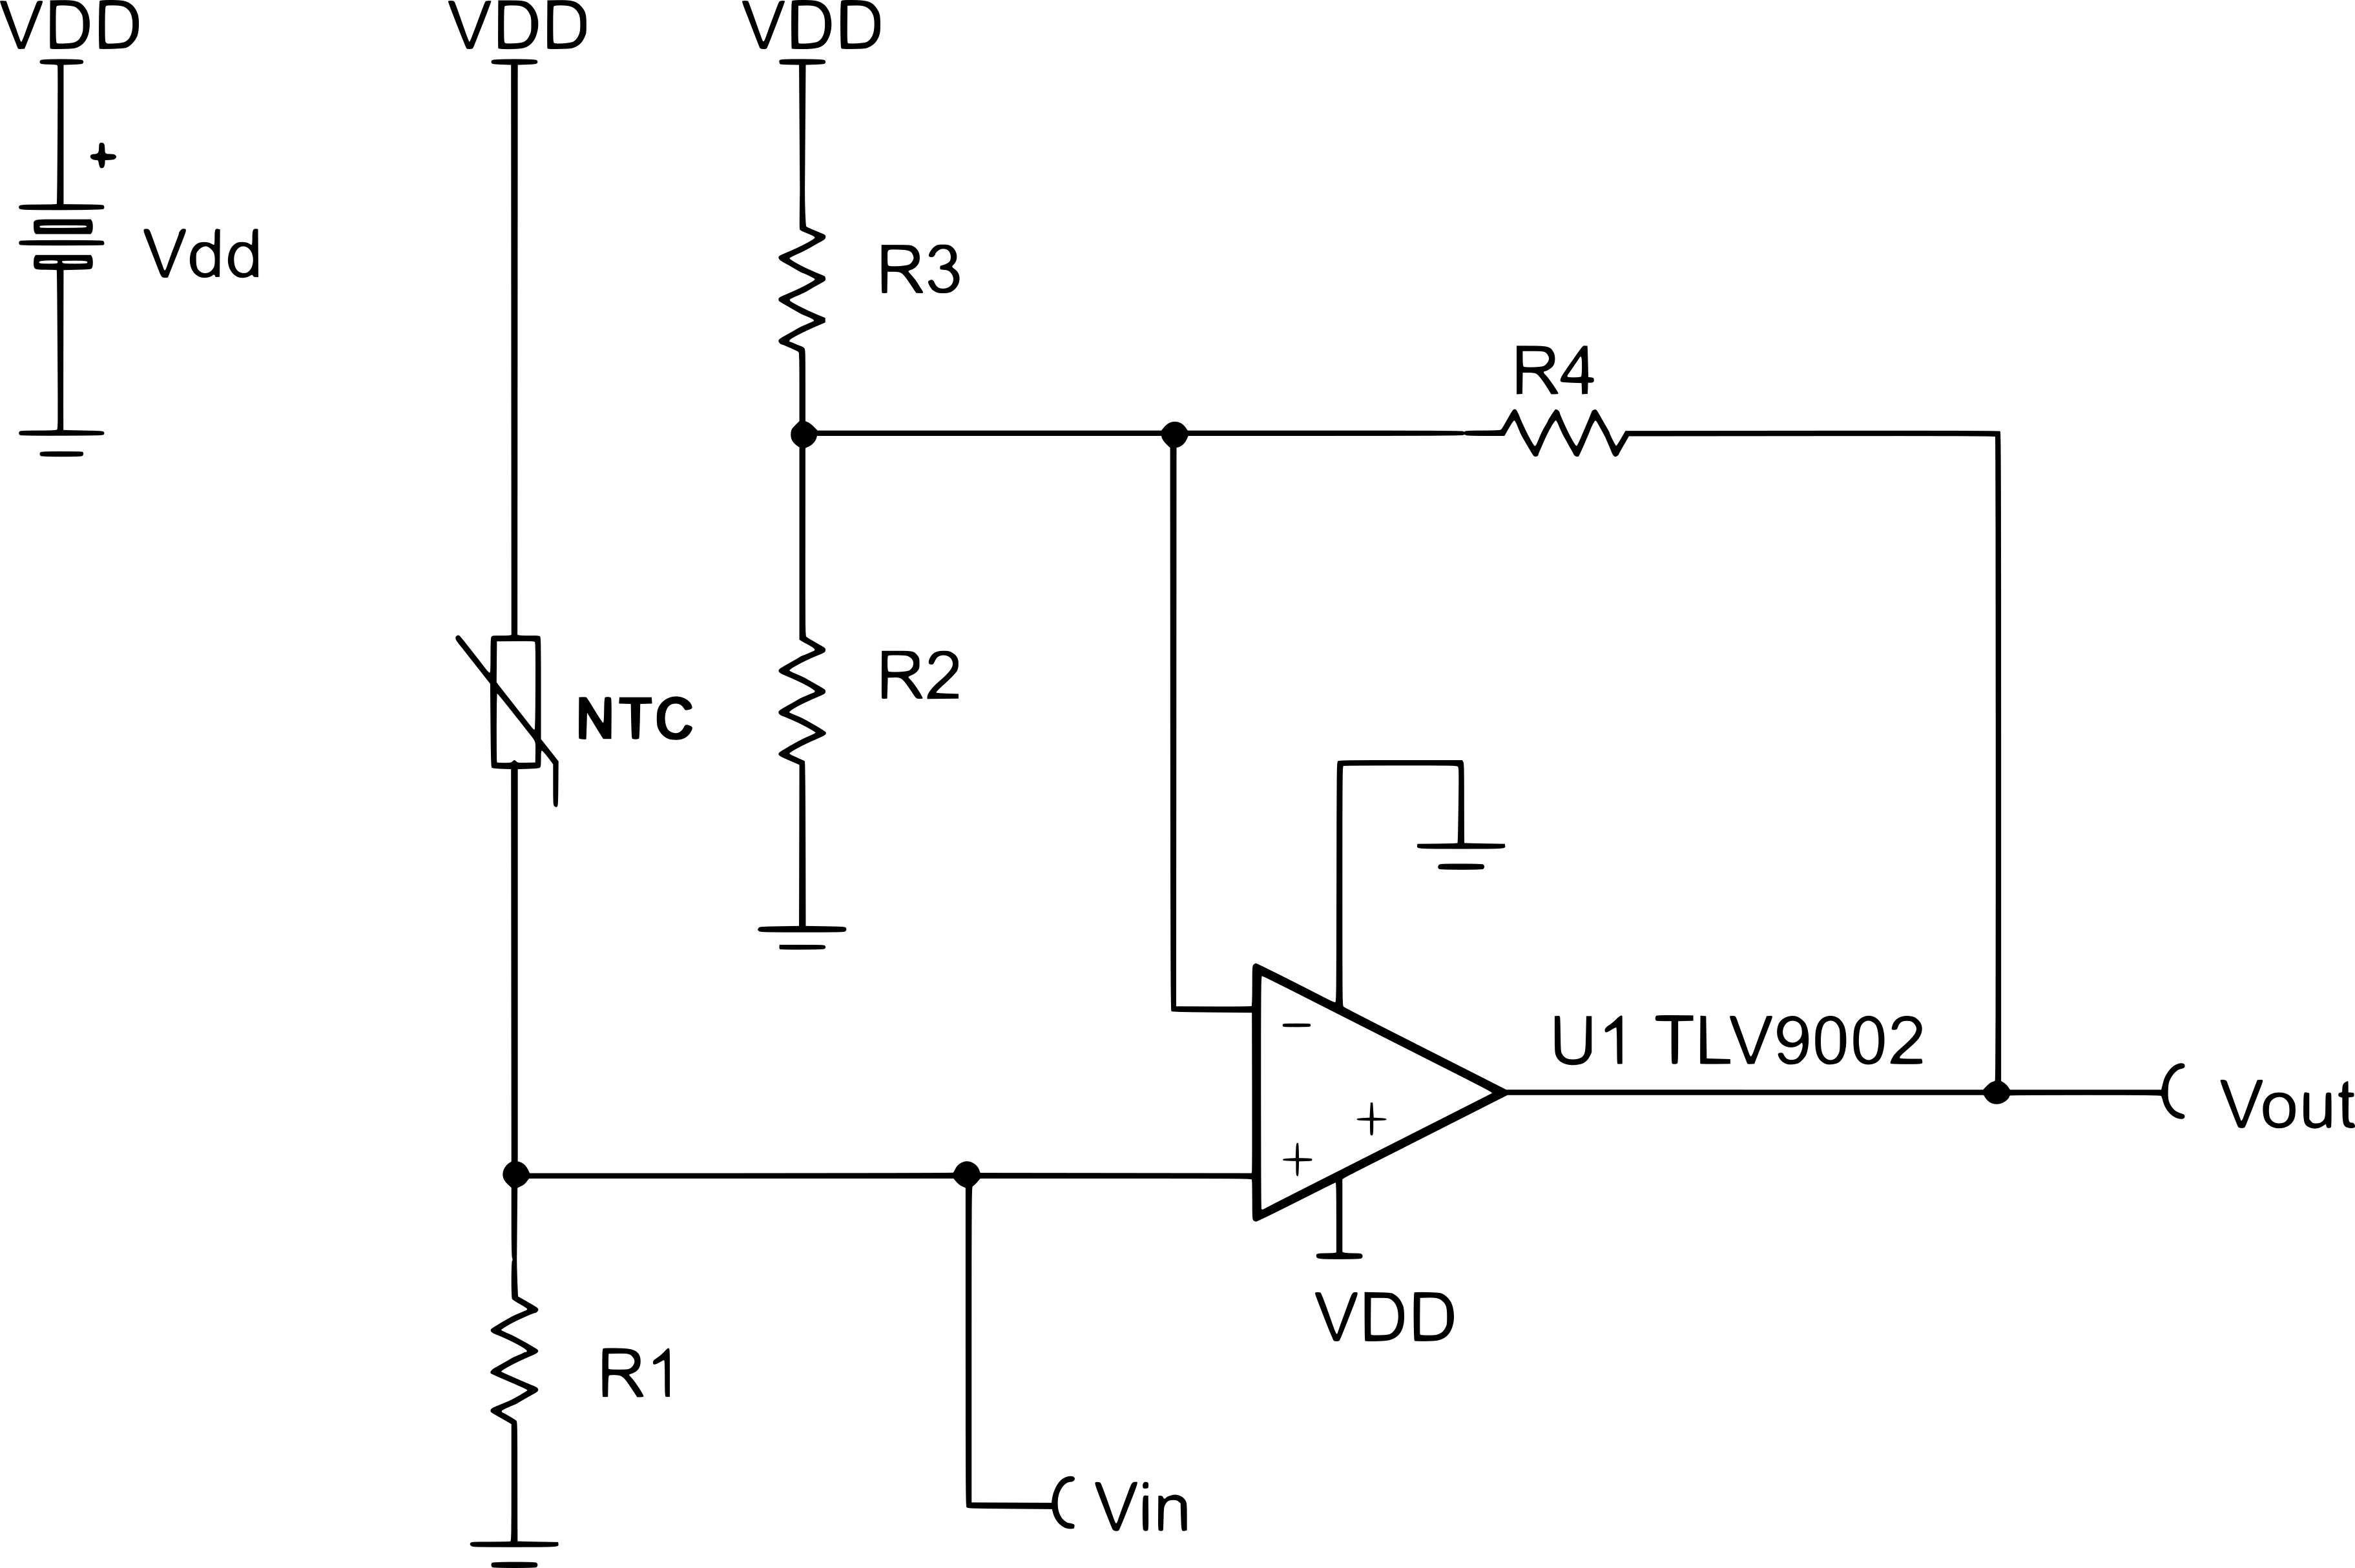
\includegraphics[width=\textwidth]{schematic.png}
  \caption{Schematic}
\end{figure}

\input{calculations.tex}

\begin{figure}[!htbp]
  \centering
  \includegraphics[width=\textwidth]{curve.png}
  \caption{Schematic}
\end{figure}

\end{document}
